\section{\label{sec:level1}Results}

We determined $\bm{\alpha_Q, E_f,}$ and $\bm{E_s}$ for each PMT. $\bm{\alpha_f}$ and $\bm{\alpha_s}$ at the four Ra 226 energy peak values, 4.8, 5.5, 6.0, and 7.7 MeV. The fast and slow proportion was also found for each PMT. For each PMT we fit every source with a Gaussian function which yielded the following parameter fits Figure \ref{fig:gaussfits}. Missing data is from trials that did not produce resolved energy peaks to fit a Gaussian. Each PMT still has enough peak values to complete the analysis. 

\begin{figure}
  \centering
    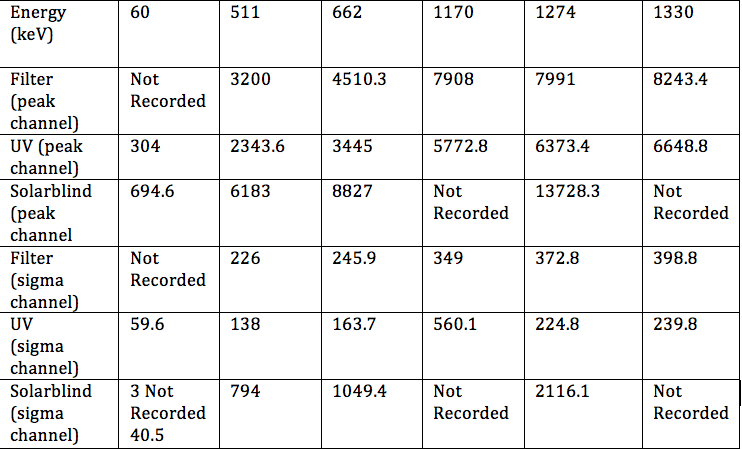
\includegraphics[width=.9\columnwidth]{gaussfits.png}
  \caption{Table with the recorded gaussian fit parameters}
  \label{fig:gaussfits}
\end{figure} 

\noindent
Using the peak value and associated sigma, the keV to channels conversion Figure \ref{fig:chanf}, Figure \ref{fig:chanuv}, and Figure \ref{fig:chansb} was determined for each PMT; 

\begin{table}
    \begin{tabular}{ | l | l | p{2cm} |}
    \hline
    PMT & Channels to keV\\ \hline

    UV with filter & 6.33012509\\ \hline  

    UV & 4.984\\ \hline

    Solarblind & 12.0694256\\ \hline
    \hline
    \end{tabular}
    \caption{These values represent the slope of the line from channels (found from the caen output) to keV (from the known values) for each PMT.}
    \label{table:chan_kev}
\end{table}

\begin{figure}
  \centering
    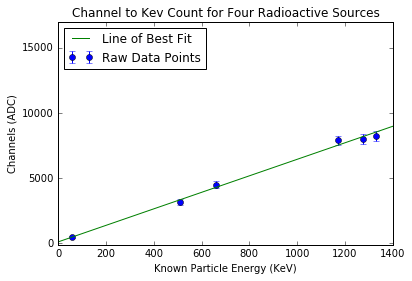
\includegraphics[width=.8\columnwidth]{chanf.png}
  \caption{UV with filter Calibration Function}
  \label{fig:chanf}
\end{figure} 

\begin{figure}
  \centering
    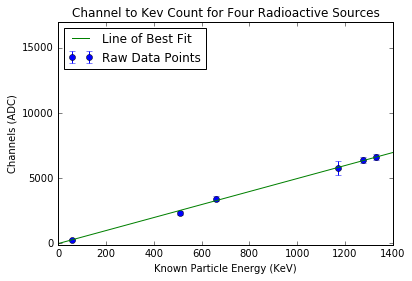
\includegraphics[width=.8\columnwidth]{chanuv.png}
  \caption{UV Calibration Function}
  \label{fig:chanuv}
\end{figure} 

\begin{figure}
  \centering
    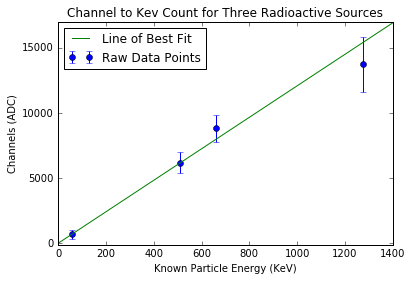
\includegraphics[width=.8\columnwidth]{chansb.png}
  \caption{Solarblind Calibration Function}
  \label{fig:chansb}
\end{figure} 

The inverse slope of the best fit line multiplied by the Ra 226 peak channel values yielded the expected energy in keV, which then determined the quenching factors $\bm{\alpha_Q}$ Figure \ref{fig:qff}, Figure \ref{fig:qfuv}, and Figure \ref{fig:qfsb}.

\begin{table}
    \begin{tabular}{ | l | l | l | l | p{2cm} |}
    \hline
    PMT & 4800 & 5500 & 6000 & 7700\\ \hline

    UV with filter & 2.976 & 2.849 & 2.704 & 2.460\\ \hline  

    UV & 3.269 & 3.136 & 2.977 & 2.702\\ \hline

    Solarblind & 5.155 & 4.789 & 4.475 & 4.166\\ \hline
    \hline
    \end{tabular}
    \caption{These values represent the quenching factor found at each energy level for eahc PMT. These were determined by comparing the expected conversion keV value with the known keV value for each Ra 226 peak}
    \label{table:quench}
\end{table}

\begin{figure}
  \centering
    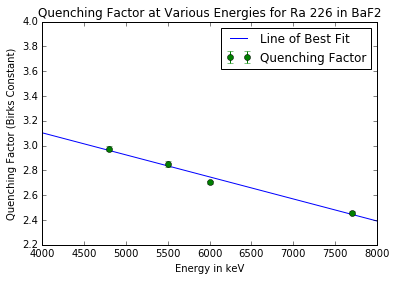
\includegraphics[width=.8\columnwidth]{qff.png}
  \caption{UV with filter Quenching Factors}
  \label{fig:qff}
\end{figure} 

\begin{figure}
  \centering
    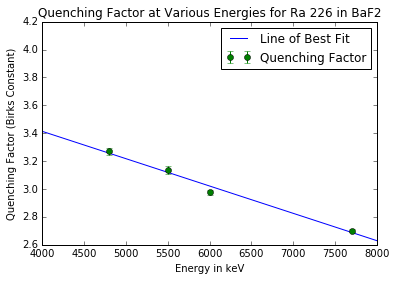
\includegraphics[width=.8\columnwidth]{qfuv.png}
  \caption{UV Quenching Factors}
  \label{fig:qfuv}
\end{figure} 

\begin{figure}
  \centering
    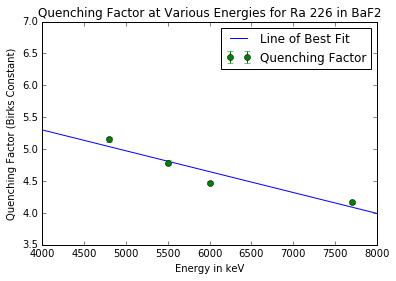
\includegraphics[width=.8\columnwidth]{qfsb.png}
  \caption{Solarblind Quenching Factors}
  \label{fig:qfsb}
\end{figure} 

The emission spectrum of Barium Fluoride was plotted and fitted with four Gaussians. Using this fit we convolved each QE spectrum Figure \ref{fig:FitsBaF2} to find $\bm{E_f}$ and $\bm{E_s}$ Figure \ref{fig:convf}, Figure \ref{fig:convuv}, and Figure \ref{fig:convsb}.

\begin{table}
    \begin{tabular}{ | l | l | p{2cm} |}
    \hline
    PMT & Fast Percentage & Slow Percentage\\ \hline

    UV with filter & 0.104 & 0.895\\ \hline  

    UV & 0.112 & 0.887\\ \hline

    Solarblind & 0.558 & 0.441\\ \hline
    \hline
    \end{tabular}
    \caption{These values represent the percentage of light that is from the fast and slow component for each PMT. They are defined as the area under the first two and last two Gaussians of the convolution of the $BaF_2$ emission spectrum and the QE of each PMT}
    \label{table:fastvsslow}
\end{table}

\begin{figure}
  \centering
    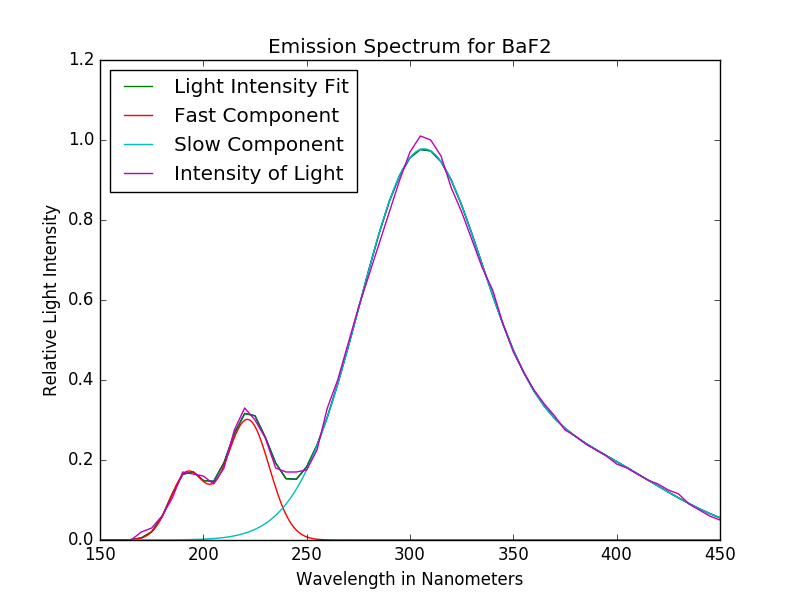
\includegraphics[width=.8\columnwidth]{FitsBaF2.png}
  \caption{Barium Fluoride emission spectrum}
  \label{fig:FitsBaF2}
\end{figure} 

\begin{figure}
  \centering
    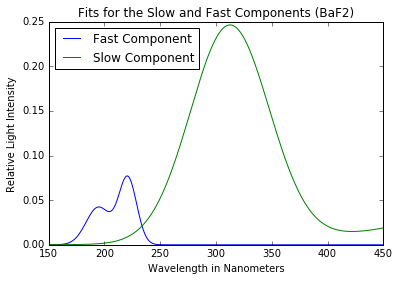
\includegraphics[width=.8\columnwidth]{convf.png}
  \caption{UV with filter Convolution}
  \label{fig:convf}
\end{figure} 

\begin{figure}
  \centering
    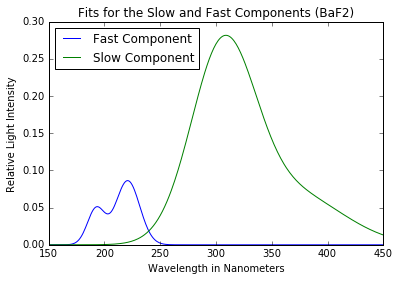
\includegraphics[width=.8\columnwidth]{convuv.png}
  \caption{UV Convolution}
  \label{fig:convuv}
\end{figure} 

\begin{figure}
  \centering
    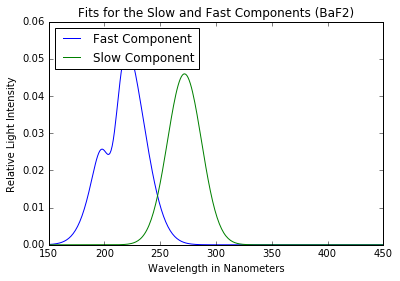
\includegraphics[width=.8\columnwidth]{convsb.png}
  \caption{Solarblind Convolution}
  \label{fig:convsb}
\end{figure} 

\noindent
We plotted our determined values in this form for every Ra 226 peak, Figure \ref{fig:first}, Figure \ref{fig:second}, Figure \ref{fig:third}, and Figure \ref{fig:fourth}, with equation (2). Solving for the point of best intersection, (\bm{$\alpha_s, \alpha_f}$), at each energy level the quenching factor as a function of energy is shown in equations (10) and (11) with respective errors in equations (12) and (13). 


\begin{align}
\bm{\alpha_s = -0.1398072 * RE_k\alpha + 4.13497323 \label{eq:ten}
\\
\alpha_f = -0.45007859 * RE_k\alpha + 11.23363402 \label{eq:eleven}}
\end{align}


\begin{table}
    \begin{tabular}{ | l | l | p{2cm} |}
    \hline
    Component Error & 4800 & 5500 & 6000 & 7700\\ \hline

    Slow Error & 1.362 & 1.310 & 1.233 & 1.109\\ \hline  

    Fast Error & 0.029 & 0.031 & 0.031 & 0.031\\ \hline
    \hline
    \end{tabular}
    \caption{These values represent the error on each fast and slow quenching factor determined from the covariance matrix in the calculation of the point of best intersection.}
    \label{table:fastvsslow}
\end{table}
 

\noindent
Figure \ref{fig:qf} shows Birk's constant as a function of energy for the fast and slow component for alpha particle interactions with Barium Fluoride crystals.

\begin{figure}
  \centering
    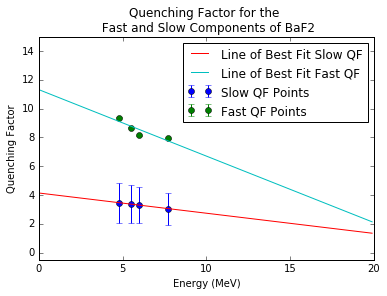
\includegraphics[width=.8\columnwidth]{qf.png}
  \caption{Final Quenching Factor Function}
  \label{fig:qf}
\end{figure} 


\section{\label{sec:level1}Discussion}


The separation of light from the fast and slow components for $BaF_2$ can be determined for any alpha particle from the measured slow and fast quenching factors. The total light from the fast component is found by solving Birk's Law, equation (1), to be a function of the integral of energy lost per distance (citation). 


The total energy is also determined using the above analysis. The integral of $\bm{dE/dx}$ is the total energy from the particle which is already known. By replacing general $\bm{\alpha_Q}$ with $\bm{\alpha_f}$ for the particles energy the light yield can be determined. 

In high energy physics experiments collaborators are trying to determine the energy or mass of a particle. Instead $\bm{dL/dx}$ is known from the calorimeter. For experiments of this nature, our measured Birk's constants will allow for precision in alpha particle discoveries using Barium Fluoride. 

\section{\label{sec:level1}Acknowledgements}
\squeezeup

The California Institute of Technology and its Student Faculty Programs office made the measurement of the quenching factor for barium fluoride crystals possible. A. Hasse would also like to express her deep gratitude towards Professor David Hitlin, Jake Kim, and Jason Trevor and the High Energy Physics group for this opportunity and their continuing support. 
\squeezeup

\section{\label{sec:level1}References}
\squeezeup

\begin{thebibliography}{9}
\bibitem{BaF2specs} 
Saint Gobain Ceramics and Plastics Inc. 
\textit{$BaF_2$ Barium Fluoride Scintillation Material}. 
2014.
 
\bibitem{Mu2e} 
Bartosvek, L., et. al.
\textit{Mu2e Technical Design Report}.
Fermi National Accelerator Laboratory. 
 
\bibitem{caen} 
CAEN SpA
\textit{Electronic Instrumentation DPSD Register Description}
\\\texttt{http://www-cs-faculty.stanford.edu/\~{}uno/abcde.html}
2013

\bibitem{scint} 
L'Annunziata, M.
\textit{Handbook of Radioactivity Analysis}.
2003

\bibitem{BaF2scint} 
Matulewicz, T.
\textit{Quenching of Scintillation in $BaF_2$ for Light Charged Particle}.
14021 Caen Cedex, France. 1967.

\bibitem{PMT} 
Hamamatsu
\textit{Photomultiplier Tubes, Basics, and Applications}.
2007

\bibitem{Ra226} 
Polischuk, O., Belli, P., Bernabei, R., Capella, F., Caracciolo, V., Cerulli, R., . . . Tretyak, V.
\textit{Radioactive contamination of BaF2 crystal scintillator}.
Nuclear Institute. 2009

\end{thebibliography}

\squeezeup

\section{\label{sec:level1}Appendix}

\subsection{\label{sec:level2}Gaussian Fits}
\squeezeup

The next three sections show all of the Gaussian fits for each PMT. 
\squeezeup

\subsubsection{\label{sec:level3}UV Extended Full Spectrum}
\squeezeup


\begin{figure*}
  \centering
  \subfloat[\label{fig:2UVAmBefit} AmBe 241 UV PMT]{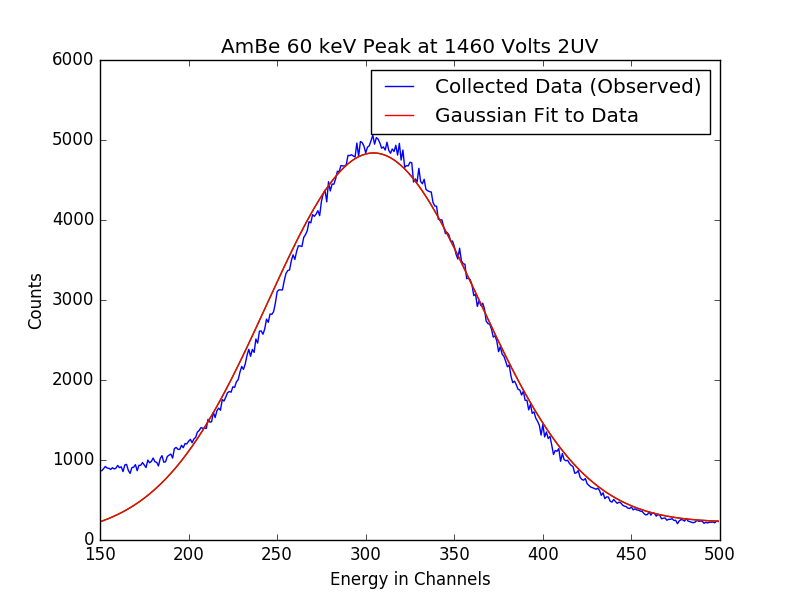
\includegraphics[width=.8\columnwidth]{2UVAmBefit.png}}%
  \qquad
  \subfloat[\label{fig:2UVCsfit} Cs 137 UV PMT]{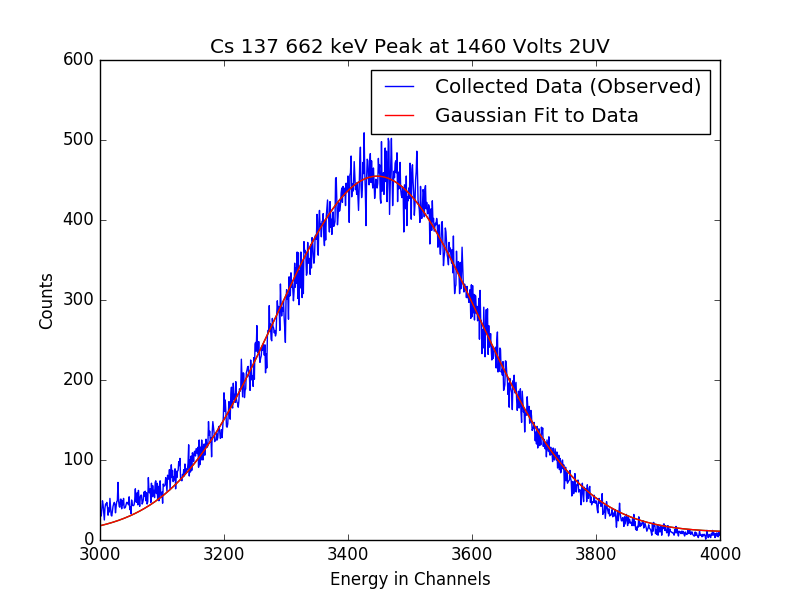
\includegraphics[width=.8\columnwidth]{2UVCsfit.png}}%
  \qquad
  \subfloat[\label{fig:2UVCo1fit} Co 60 Peak 1 UV PMT]{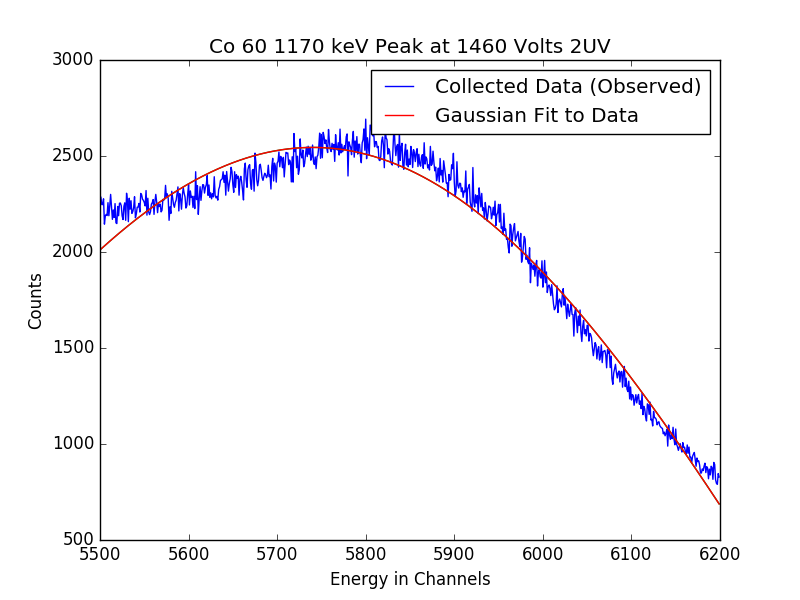
\includegraphics[width=.8\columnwidth]{2UVCo1fit.png}}%
  \qquad
  \subfloat[\label{fig:2UVCo2fit} Co 60 Peak 2 UV PMT]{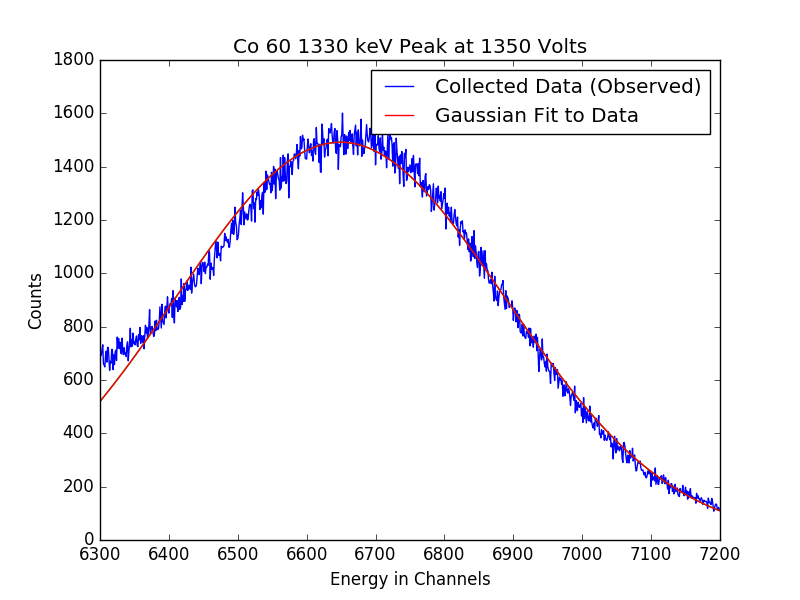
\includegraphics[width=.8\columnwidth]{2UVCo2fit.png}}%
  \qquad
  \subfloat[\label{fig:2UVNa1fit} Na 22 Peak 1 UV PMT]{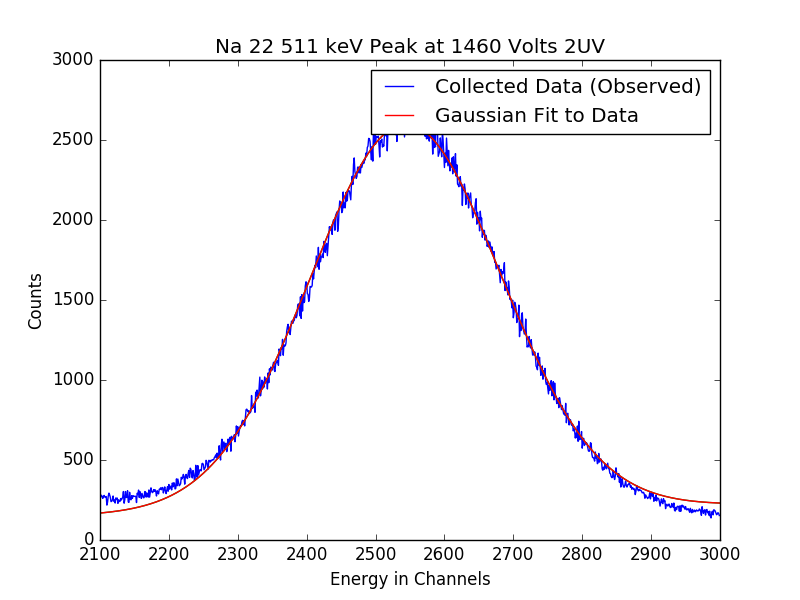
\includegraphics[width=.8\columnwidth]{2UVNa1fit.png}}%
  \qquad
  \subfloat[\label{fig:2UVNa2fit} Na 22 Peak 2 UV PMT]{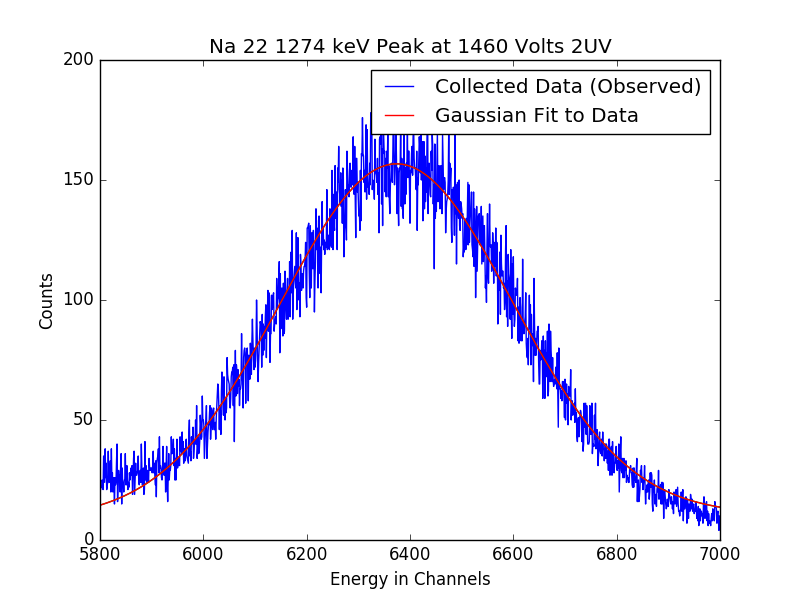
\includegraphics[width=.8\columnwidth]{2UVNa2fit.png}}%
  \qquad
  \subfloat[\label{fig:2UVRa1fit} Ra 226 First Three Peaks UV PMT]{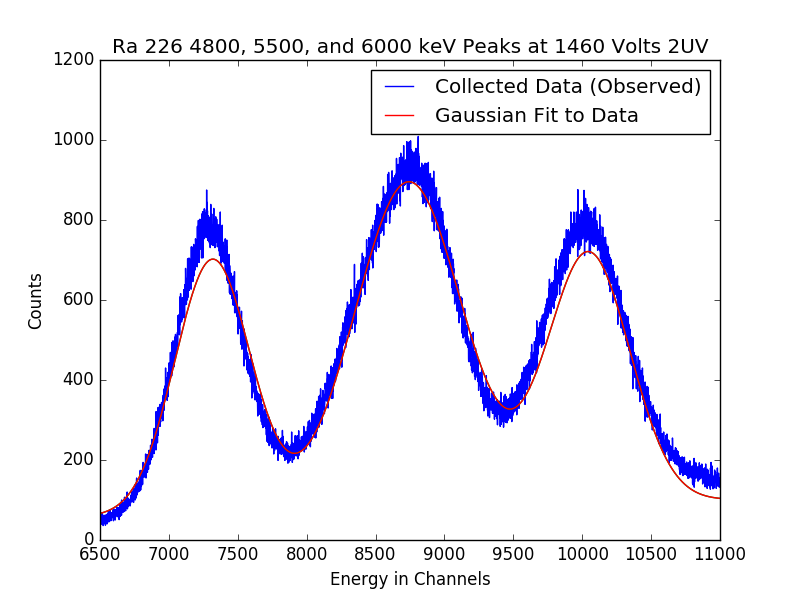
\includegraphics[width=.8\columnwidth]{2UVRa1fit.png}}%
  \qquad
  \subfloat[\label{fig:2UVRa4fit} Ra 226 Fourth Peak UV PMT]{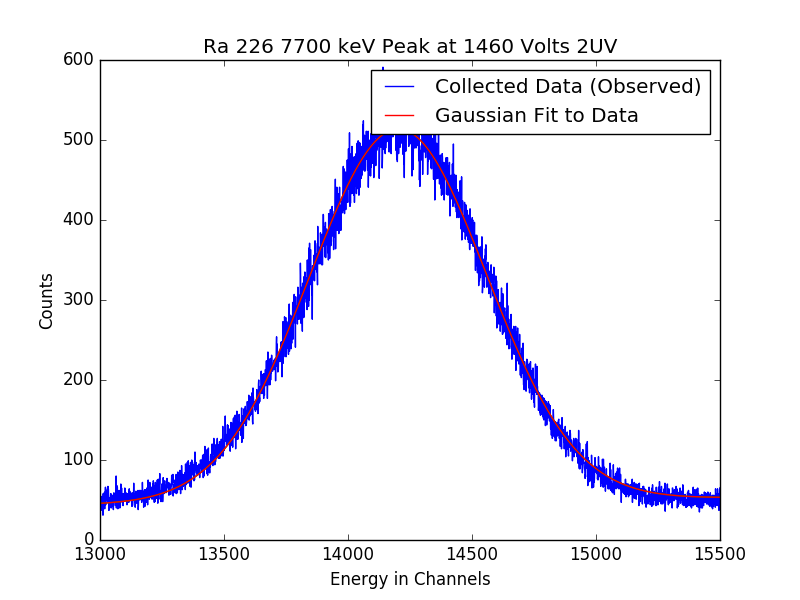
\includegraphics[width=.8\columnwidth]{2UVRa4fit.png}}%
  \qquad
\caption{ha}
\end{figure*}